\documentclass[twoside,openright,titlepage,numbers=noenddot,headinclude,%
               footinclude=true,cleardoublepage=empty,abstractoff,BCOR=5mm,%
               paper=a4,fontsize=11pt,ngerman,american]{scrreprt}

% Custom config ===============================================================

% Classic thesis
\usepackage{amssymb}
% ****************************************************************************************************
% classicthesis-config.tex
% formerly known as loadpackages.sty, classicthesis-ldpkg.sty, and classicthesis-preamble.sty
% Use it at the beginning of your ClassicThesis.tex, or as a LaTeX Preamble
% in your ClassicThesis.{tex,lyx} with % ****************************************************************************************************
% classicthesis-config.tex
% formerly known as loadpackages.sty, classicthesis-ldpkg.sty, and classicthesis-preamble.sty
% Use it at the beginning of your ClassicThesis.tex, or as a LaTeX Preamble
% in your ClassicThesis.{tex,lyx} with % ****************************************************************************************************
% classicthesis-config.tex
% formerly known as loadpackages.sty, classicthesis-ldpkg.sty, and classicthesis-preamble.sty
% Use it at the beginning of your ClassicThesis.tex, or as a LaTeX Preamble
% in your ClassicThesis.{tex,lyx} with \input{classicthesis-config}
% ****************************************************************************************************
% If you like the classicthesis, then I would appreciate a postcard.
% My address can be found in the file ClassicThesis.pdf. A collection
% of the postcards I received so far is available online at
% http://postcards.miede.de
% ****************************************************************************************************

% ****************************************************************************************************
% 1. Configure classicthesis for your needs here, e.g., remove "drafting" below
% in order to deactivate the time-stamp on the pages
% ****************************************************************************************************
\PassOptionsToPackage{listings,%drafting,% %eulerchapternumbers,%
				 pdfspacing,eulermath,%floatperchapter,%linedheaders,%
				 subfig,parts,dottedtoc}{classicthesis}
% ********************************************************************
% Available options for classicthesis.sty
% (see ClassicThesis.pdf for more information):
% drafting
% parts nochapters linedheaders
% eulerchapternumbers beramono eulermath pdfspacing minionprospacing
% tocaligned dottedtoc manychapters
% listings floatperchapter subfig
% ********************************************************************

% ********************************************************************
% Triggers for this config
% ********************************************************************
\usepackage{ifthen}
\newboolean{enable-backrefs} % enable backrefs in the bibliography
\setboolean{enable-backrefs}{false} % true false
% ****************************************************************************************************


% ****************************************************************************************************
% 2. Personal data and user ad-hoc commands
% ****************************************************************************************************
\newcommand{\myTitle}{Understanding Random Forests\xspace}
\newcommand{\mySubtitle}{From Theory to Practice\xspace}
\newcommand{\myDegree}{Doktor-Ingenieur (Dr.-Ing.)\xspace}
\newcommand{\myName}{Gilles Louppe\xspace}
\newcommand{\myProf}{Put name here\xspace}
\newcommand{\myOtherProf}{Put name here\xspace}
\newcommand{\mySupervisor}{Pierre Geurts\xspace}
\newcommand{\myFaculty}{Faculty of Applied Sciences\xspace}
\newcommand{\myDepartment}{Department of EE and CS\xspace}
\newcommand{\myUni}{University of Liege\xspace}
\newcommand{\myLocation}{Liege, Belgium\xspace}
\newcommand{\myTime}{June 2014\xspace}
\newcommand{\myVersion}{version 1.0\xspace}

% ********************************************************************
% Setup, finetuning, and useful commands
% ********************************************************************
\newcounter{dummy} % necessary for correct hyperlinks (to index, bib, etc.)
\newlength{\abcd} % for ab..z string length calculation
\providecommand{\mLyX}{L\kern-.1667em\lower.25em\hbox{Y}\kern-.125emX\@}
\newcommand{\ie}{i.\,e.}
\newcommand{\Ie}{I.\,e.}
\newcommand{\eg}{e.\,g.}
\newcommand{\Eg}{E.\,g.}
% ****************************************************************************************************


% ****************************************************************************************************
% 3. Loading some handy packages
% ****************************************************************************************************
% ********************************************************************
% Packages with options that might require adjustments
% ********************************************************************
%\PassOptionsToPackage{latin9}{inputenc}	% latin9 (ISO-8859-9) = latin1+"Euro sign"
% \usepackage{inputenc}

\usepackage[applemac]{inputenc}

%\PassOptionsToPackage{ngerman,american}{babel}   % change this to your language(s)
% Spanish languages need extra options in order to work with this template
%\PassOptionsToPackage{spanish,es-lcroman}{babel}
 \usepackage{babel}

\PassOptionsToPackage{square,authoryear}{natbib}
 \usepackage{natbib}

\PassOptionsToPackage{fleqn}{amsmath}		% math environments and more by the AMS
 \usepackage{amsmath}

% ********************************************************************
% General useful packages
% ********************************************************************
\PassOptionsToPackage{T1}{fontenc} % T2A for cyrillics
	\usepackage{fontenc}


\usepackage{lipsum}
\usepackage{textcomp} % fix warning with missing font shapes
%\usepackage{scrhack} % fix warnings when using KOMA with listings package
\usepackage{xspace} % to get the spacing after macros right
\usepackage{mparhack} % get marginpar right
\usepackage{fixltx2e} % fixes some LaTeX stuff
\PassOptionsToPackage{printonlyused,smaller}{acronym}
	\usepackage{acronym} % nice macros for handling all acronyms in the thesis
%\renewcommand*{\acsfont}[1]{\textssc{#1}} % for MinionPro
%\renewcommand{\bflabel}[1]{{#1}\hfill} % fix the list of acronyms
% ****************************************************************************************************


% ****************************************************************************************************
% 4. Setup floats: tables, (sub)figures, and captions
% ****************************************************************************************************
\usepackage{tabularx} % better tables
	\setlength{\extrarowheight}{3pt} % increase table row height
\newcommand{\tableheadline}[1]{\multicolumn{1}{c}{\spacedlowsmallcaps{#1}}}
\newcommand{\myfloatalign}{\centering} % to be used with each float for alignment
\usepackage{caption}
\captionsetup{format=hang,font=small}
\usepackage{subfig}
% ****************************************************************************************************


% ****************************************************************************************************
% 5. Setup code listings
% ****************************************************************************************************
\usepackage{listings}
%\lstset{emph={trueIndex,root},emphstyle=\color{BlueViolet}}%\underbar} % for special keywords
\lstset{language=[LaTeX]Tex,%C++,
    keywordstyle=\color{RoyalBlue},%\bfseries,
    basicstyle=\small\ttfamily,
    %identifierstyle=\color{NavyBlue},
    commentstyle=\color{Green}\ttfamily,
    stringstyle=\rmfamily,
    numbers=none,%left,%
    numberstyle=\scriptsize,%\tiny
    stepnumber=5,
    numbersep=8pt,
    showstringspaces=false,
    breaklines=true,
    frameround=ftff,
    frame=single,
    belowcaptionskip=.75\baselineskip
    %frame=L
}
% ****************************************************************************************************


% ****************************************************************************************************
% 6. PDFLaTeX, hyperreferences and citation backreferences
% ****************************************************************************************************
% ********************************************************************
% Using PDFLaTeX
% ********************************************************************
\PassOptionsToPackage{pdftex,hyperfootnotes=true,pdfpagelabels}{hyperref}
	\usepackage{hyperref}  % backref linktocpage pagebackref
\pdfcompresslevel=9
\pdfadjustspacing=1
\PassOptionsToPackage{pdftex}{graphicx}
	\usepackage{graphicx}

% ********************************************************************
% Setup the style of the backrefs from the bibliography
% (translate the options to any language you use)
% ********************************************************************
\newcommand{\backrefnotcitedstring}{\relax}%(Not cited.)
\newcommand{\backrefcitedsinglestring}[1]{(Cited on page~#1.)}
\newcommand{\backrefcitedmultistring}[1]{(Cited on pages~#1.)}
\ifthenelse{\boolean{enable-backrefs}}%
{%
		\PassOptionsToPackage{hyperpageref}{backref}
		\usepackage{backref} % to be loaded after hyperref package
		   \renewcommand{\backreftwosep}{ and~} % separate 2 pages
		   \renewcommand{\backreflastsep}{, and~} % separate last of longer list
		   \renewcommand*{\backref}[1]{}  % disable standard
		   \renewcommand*{\backrefalt}[4]{% detailed backref
		      \ifcase #1 %
		         \backrefnotcitedstring%
		      \or%
		         \backrefcitedsinglestring{#2}%
		      \else%
		         \backrefcitedmultistring{#2}%
		      \fi}%
}{\relax}

% ********************************************************************
% Hyperreferences
% ********************************************************************
\hypersetup{%
    %draft,	% = no hyperlinking at all (useful in b/w printouts)
    colorlinks=true, linktocpage=true, pdfstartpage=3, pdfstartview=FitV,%
    % uncomment the following line if you want to have black links (e.g., for printing)
    %colorlinks=false, linktocpage=false, pdfborder={0 0 0}, pdfstartpage=3, pdfstartview=FitV,%
    breaklinks=true, pdfpagemode=UseNone, pageanchor=true, pdfpagemode=UseOutlines,%
    plainpages=false, bookmarksnumbered, bookmarksopen=true, bookmarksopenlevel=1,%
    hypertexnames=true, pdfhighlight=/O,%nesting=true,%frenchlinks,%
    urlcolor=webbrown, linkcolor=RoyalBlue, citecolor=webgreen, %pagecolor=RoyalBlue,%
    %urlcolor=Black, linkcolor=Black, citecolor=Black, %pagecolor=Black,%
    pdftitle={\myTitle},%
    pdfauthor={\textcopyright\ \myName, \myUni, \myFaculty},%
    pdfsubject={},%
    pdfkeywords={},%
    pdfcreator={pdfLaTeX},%
    pdfproducer={LaTeX with hyperref and classicthesis}%
}

% ********************************************************************
% Setup autoreferences
% ********************************************************************
% There are some issues regarding autorefnames
% http://www.ureader.de/msg/136221647.aspx
% http://www.tex.ac.uk/cgi-bin/texfaq2html?label=latexwords
% you have to redefine the makros for the
% language you use, e.g., american, ngerman
% (as chosen when loading babel/AtBeginDocument)
% ********************************************************************
\makeatletter
\@ifpackageloaded{babel}%
    {%
       \addto\extrasamerican{%
					\renewcommand*{\figureautorefname}{Figure}%
					\renewcommand*{\tableautorefname}{Table}%
					\renewcommand*{\partautorefname}{Part}%
					\renewcommand*{\chapterautorefname}{Chapter}%
					\renewcommand*{\sectionautorefname}{Section}%
					\renewcommand*{\subsectionautorefname}{Section}%
					\renewcommand*{\subsubsectionautorefname}{Section}%
				}%
       \addto\extrasngerman{%
					\renewcommand*{\paragraphautorefname}{Absatz}%
					\renewcommand*{\subparagraphautorefname}{Unterabsatz}%
					\renewcommand*{\footnoteautorefname}{Fu\"snote}%
					\renewcommand*{\FancyVerbLineautorefname}{Zeile}%
					\renewcommand*{\theoremautorefname}{Theorem}%
					\renewcommand*{\appendixautorefname}{Anhang}%
					\renewcommand*{\equationautorefname}{Gleichung}%
					\renewcommand*{\itemautorefname}{Punkt}%
				}%
			% Fix to getting autorefs for subfigures right (thanks to Belinda Vogt for changing the definition)
			\providecommand{\subfigureautorefname}{\figureautorefname}%
    }{\relax}
\makeatother


% ****************************************************************************************************
% 7. Last calls before the bar closes
% ****************************************************************************************************
% ********************************************************************
% Development Stuff
% ********************************************************************
\listfiles
%\PassOptionsToPackage{l2tabu,orthodox,abort}{nag}
%	\usepackage{nag}
%\PassOptionsToPackage{warning, all}{onlyamsmath}
%	\usepackage{onlyamsmath}

% ********************************************************************
% Last, but not least...
% ********************************************************************
\usepackage{classicthesis}
% ****************************************************************************************************


% ****************************************************************************************************
% 8. Further adjustments (experimental)
% ****************************************************************************************************
% ********************************************************************
% Changing the text area
% ********************************************************************
%\linespread{1.05} % a bit more for Palatino
%\areaset[current]{312pt}{761pt} % 686 (factor 2.2) + 33 head + 42 head \the\footskip
%\setlength{\marginparwidth}{7em}%
%\setlength{\marginparsep}{2em}%

% ********************************************************************
% Using different fonts
% ********************************************************************
%\usepackage[oldstylenums]{kpfonts} % oldstyle notextcomp
%\usepackage[osf]{libertine}
%\usepackage{hfoldsty} % Computer Modern with osf
%\usepackage[light,condensed,math]{iwona}
%\renewcommand{\sfdefault}{iwona}
%\usepackage{lmodern} % <-- no osf support :-(
% \usepackage[T1]{fontenc}
% \usepackage{textcomp}
%\usepackage[urw-garamond]{mathdesign} <-- no osf support :-(
% ****************************************************************************************************

% ****************************************************************************************************
% If you like the classicthesis, then I would appreciate a postcard.
% My address can be found in the file ClassicThesis.pdf. A collection
% of the postcards I received so far is available online at
% http://postcards.miede.de
% ****************************************************************************************************

% ****************************************************************************************************
% 1. Configure classicthesis for your needs here, e.g., remove "drafting" below
% in order to deactivate the time-stamp on the pages
% ****************************************************************************************************
\PassOptionsToPackage{listings,%drafting,% %eulerchapternumbers,%
				 pdfspacing,eulermath,%floatperchapter,%linedheaders,%
				 subfig,parts,dottedtoc}{classicthesis}
% ********************************************************************
% Available options for classicthesis.sty
% (see ClassicThesis.pdf for more information):
% drafting
% parts nochapters linedheaders
% eulerchapternumbers beramono eulermath pdfspacing minionprospacing
% tocaligned dottedtoc manychapters
% listings floatperchapter subfig
% ********************************************************************

% ********************************************************************
% Triggers for this config
% ********************************************************************
\usepackage{ifthen}
\newboolean{enable-backrefs} % enable backrefs in the bibliography
\setboolean{enable-backrefs}{false} % true false
% ****************************************************************************************************


% ****************************************************************************************************
% 2. Personal data and user ad-hoc commands
% ****************************************************************************************************
\newcommand{\myTitle}{Understanding Random Forests\xspace}
\newcommand{\mySubtitle}{From Theory to Practice\xspace}
\newcommand{\myDegree}{Doktor-Ingenieur (Dr.-Ing.)\xspace}
\newcommand{\myName}{Gilles Louppe\xspace}
\newcommand{\myProf}{Put name here\xspace}
\newcommand{\myOtherProf}{Put name here\xspace}
\newcommand{\mySupervisor}{Pierre Geurts\xspace}
\newcommand{\myFaculty}{Faculty of Applied Sciences\xspace}
\newcommand{\myDepartment}{Department of EE and CS\xspace}
\newcommand{\myUni}{University of Liege\xspace}
\newcommand{\myLocation}{Liege, Belgium\xspace}
\newcommand{\myTime}{June 2014\xspace}
\newcommand{\myVersion}{version 1.0\xspace}

% ********************************************************************
% Setup, finetuning, and useful commands
% ********************************************************************
\newcounter{dummy} % necessary for correct hyperlinks (to index, bib, etc.)
\newlength{\abcd} % for ab..z string length calculation
\providecommand{\mLyX}{L\kern-.1667em\lower.25em\hbox{Y}\kern-.125emX\@}
\newcommand{\ie}{i.\,e.}
\newcommand{\Ie}{I.\,e.}
\newcommand{\eg}{e.\,g.}
\newcommand{\Eg}{E.\,g.}
% ****************************************************************************************************


% ****************************************************************************************************
% 3. Loading some handy packages
% ****************************************************************************************************
% ********************************************************************
% Packages with options that might require adjustments
% ********************************************************************
%\PassOptionsToPackage{latin9}{inputenc}	% latin9 (ISO-8859-9) = latin1+"Euro sign"
% \usepackage{inputenc}

\usepackage[applemac]{inputenc}

%\PassOptionsToPackage{ngerman,american}{babel}   % change this to your language(s)
% Spanish languages need extra options in order to work with this template
%\PassOptionsToPackage{spanish,es-lcroman}{babel}
 \usepackage{babel}

\PassOptionsToPackage{square,authoryear}{natbib}
 \usepackage{natbib}

\PassOptionsToPackage{fleqn}{amsmath}		% math environments and more by the AMS
 \usepackage{amsmath}

% ********************************************************************
% General useful packages
% ********************************************************************
\PassOptionsToPackage{T1}{fontenc} % T2A for cyrillics
	\usepackage{fontenc}


\usepackage{lipsum}
\usepackage{textcomp} % fix warning with missing font shapes
%\usepackage{scrhack} % fix warnings when using KOMA with listings package
\usepackage{xspace} % to get the spacing after macros right
\usepackage{mparhack} % get marginpar right
\usepackage{fixltx2e} % fixes some LaTeX stuff
\PassOptionsToPackage{printonlyused,smaller}{acronym}
	\usepackage{acronym} % nice macros for handling all acronyms in the thesis
%\renewcommand*{\acsfont}[1]{\textssc{#1}} % for MinionPro
%\renewcommand{\bflabel}[1]{{#1}\hfill} % fix the list of acronyms
% ****************************************************************************************************


% ****************************************************************************************************
% 4. Setup floats: tables, (sub)figures, and captions
% ****************************************************************************************************
\usepackage{tabularx} % better tables
	\setlength{\extrarowheight}{3pt} % increase table row height
\newcommand{\tableheadline}[1]{\multicolumn{1}{c}{\spacedlowsmallcaps{#1}}}
\newcommand{\myfloatalign}{\centering} % to be used with each float for alignment
\usepackage{caption}
\captionsetup{format=hang,font=small}
\usepackage{subfig}
% ****************************************************************************************************


% ****************************************************************************************************
% 5. Setup code listings
% ****************************************************************************************************
\usepackage{listings}
%\lstset{emph={trueIndex,root},emphstyle=\color{BlueViolet}}%\underbar} % for special keywords
\lstset{language=[LaTeX]Tex,%C++,
    keywordstyle=\color{RoyalBlue},%\bfseries,
    basicstyle=\small\ttfamily,
    %identifierstyle=\color{NavyBlue},
    commentstyle=\color{Green}\ttfamily,
    stringstyle=\rmfamily,
    numbers=none,%left,%
    numberstyle=\scriptsize,%\tiny
    stepnumber=5,
    numbersep=8pt,
    showstringspaces=false,
    breaklines=true,
    frameround=ftff,
    frame=single,
    belowcaptionskip=.75\baselineskip
    %frame=L
}
% ****************************************************************************************************


% ****************************************************************************************************
% 6. PDFLaTeX, hyperreferences and citation backreferences
% ****************************************************************************************************
% ********************************************************************
% Using PDFLaTeX
% ********************************************************************
\PassOptionsToPackage{pdftex,hyperfootnotes=true,pdfpagelabels}{hyperref}
	\usepackage{hyperref}  % backref linktocpage pagebackref
\pdfcompresslevel=9
\pdfadjustspacing=1
\PassOptionsToPackage{pdftex}{graphicx}
	\usepackage{graphicx}

% ********************************************************************
% Setup the style of the backrefs from the bibliography
% (translate the options to any language you use)
% ********************************************************************
\newcommand{\backrefnotcitedstring}{\relax}%(Not cited.)
\newcommand{\backrefcitedsinglestring}[1]{(Cited on page~#1.)}
\newcommand{\backrefcitedmultistring}[1]{(Cited on pages~#1.)}
\ifthenelse{\boolean{enable-backrefs}}%
{%
		\PassOptionsToPackage{hyperpageref}{backref}
		\usepackage{backref} % to be loaded after hyperref package
		   \renewcommand{\backreftwosep}{ and~} % separate 2 pages
		   \renewcommand{\backreflastsep}{, and~} % separate last of longer list
		   \renewcommand*{\backref}[1]{}  % disable standard
		   \renewcommand*{\backrefalt}[4]{% detailed backref
		      \ifcase #1 %
		         \backrefnotcitedstring%
		      \or%
		         \backrefcitedsinglestring{#2}%
		      \else%
		         \backrefcitedmultistring{#2}%
		      \fi}%
}{\relax}

% ********************************************************************
% Hyperreferences
% ********************************************************************
\hypersetup{%
    %draft,	% = no hyperlinking at all (useful in b/w printouts)
    colorlinks=true, linktocpage=true, pdfstartpage=3, pdfstartview=FitV,%
    % uncomment the following line if you want to have black links (e.g., for printing)
    %colorlinks=false, linktocpage=false, pdfborder={0 0 0}, pdfstartpage=3, pdfstartview=FitV,%
    breaklinks=true, pdfpagemode=UseNone, pageanchor=true, pdfpagemode=UseOutlines,%
    plainpages=false, bookmarksnumbered, bookmarksopen=true, bookmarksopenlevel=1,%
    hypertexnames=true, pdfhighlight=/O,%nesting=true,%frenchlinks,%
    urlcolor=webbrown, linkcolor=RoyalBlue, citecolor=webgreen, %pagecolor=RoyalBlue,%
    %urlcolor=Black, linkcolor=Black, citecolor=Black, %pagecolor=Black,%
    pdftitle={\myTitle},%
    pdfauthor={\textcopyright\ \myName, \myUni, \myFaculty},%
    pdfsubject={},%
    pdfkeywords={},%
    pdfcreator={pdfLaTeX},%
    pdfproducer={LaTeX with hyperref and classicthesis}%
}

% ********************************************************************
% Setup autoreferences
% ********************************************************************
% There are some issues regarding autorefnames
% http://www.ureader.de/msg/136221647.aspx
% http://www.tex.ac.uk/cgi-bin/texfaq2html?label=latexwords
% you have to redefine the makros for the
% language you use, e.g., american, ngerman
% (as chosen when loading babel/AtBeginDocument)
% ********************************************************************
\makeatletter
\@ifpackageloaded{babel}%
    {%
       \addto\extrasamerican{%
					\renewcommand*{\figureautorefname}{Figure}%
					\renewcommand*{\tableautorefname}{Table}%
					\renewcommand*{\partautorefname}{Part}%
					\renewcommand*{\chapterautorefname}{Chapter}%
					\renewcommand*{\sectionautorefname}{Section}%
					\renewcommand*{\subsectionautorefname}{Section}%
					\renewcommand*{\subsubsectionautorefname}{Section}%
				}%
       \addto\extrasngerman{%
					\renewcommand*{\paragraphautorefname}{Absatz}%
					\renewcommand*{\subparagraphautorefname}{Unterabsatz}%
					\renewcommand*{\footnoteautorefname}{Fu\"snote}%
					\renewcommand*{\FancyVerbLineautorefname}{Zeile}%
					\renewcommand*{\theoremautorefname}{Theorem}%
					\renewcommand*{\appendixautorefname}{Anhang}%
					\renewcommand*{\equationautorefname}{Gleichung}%
					\renewcommand*{\itemautorefname}{Punkt}%
				}%
			% Fix to getting autorefs for subfigures right (thanks to Belinda Vogt for changing the definition)
			\providecommand{\subfigureautorefname}{\figureautorefname}%
    }{\relax}
\makeatother


% ****************************************************************************************************
% 7. Last calls before the bar closes
% ****************************************************************************************************
% ********************************************************************
% Development Stuff
% ********************************************************************
\listfiles
%\PassOptionsToPackage{l2tabu,orthodox,abort}{nag}
%	\usepackage{nag}
%\PassOptionsToPackage{warning, all}{onlyamsmath}
%	\usepackage{onlyamsmath}

% ********************************************************************
% Last, but not least...
% ********************************************************************
\usepackage{classicthesis}
% ****************************************************************************************************


% ****************************************************************************************************
% 8. Further adjustments (experimental)
% ****************************************************************************************************
% ********************************************************************
% Changing the text area
% ********************************************************************
%\linespread{1.05} % a bit more for Palatino
%\areaset[current]{312pt}{761pt} % 686 (factor 2.2) + 33 head + 42 head \the\footskip
%\setlength{\marginparwidth}{7em}%
%\setlength{\marginparsep}{2em}%

% ********************************************************************
% Using different fonts
% ********************************************************************
%\usepackage[oldstylenums]{kpfonts} % oldstyle notextcomp
%\usepackage[osf]{libertine}
%\usepackage{hfoldsty} % Computer Modern with osf
%\usepackage[light,condensed,math]{iwona}
%\renewcommand{\sfdefault}{iwona}
%\usepackage{lmodern} % <-- no osf support :-(
% \usepackage[T1]{fontenc}
% \usepackage{textcomp}
%\usepackage[urw-garamond]{mathdesign} <-- no osf support :-(
% ****************************************************************************************************

% ****************************************************************************************************
% If you like the classicthesis, then I would appreciate a postcard.
% My address can be found in the file ClassicThesis.pdf. A collection
% of the postcards I received so far is available online at
% http://postcards.miede.de
% ****************************************************************************************************

% ****************************************************************************************************
% 1. Configure classicthesis for your needs here, e.g., remove "drafting" below
% in order to deactivate the time-stamp on the pages
% ****************************************************************************************************
\PassOptionsToPackage{listings,%drafting,% %eulerchapternumbers,%
				 pdfspacing,eulermath,%floatperchapter,%linedheaders,%
				 subfig,parts,dottedtoc}{classicthesis}
% ********************************************************************
% Available options for classicthesis.sty
% (see ClassicThesis.pdf for more information):
% drafting
% parts nochapters linedheaders
% eulerchapternumbers beramono eulermath pdfspacing minionprospacing
% tocaligned dottedtoc manychapters
% listings floatperchapter subfig
% ********************************************************************

% ********************************************************************
% Triggers for this config
% ********************************************************************
\usepackage{ifthen}
\newboolean{enable-backrefs} % enable backrefs in the bibliography
\setboolean{enable-backrefs}{false} % true false
% ****************************************************************************************************


% ****************************************************************************************************
% 2. Personal data and user ad-hoc commands
% ****************************************************************************************************
\newcommand{\myTitle}{Understanding Random Forests\xspace}
\newcommand{\mySubtitle}{From Theory to Practice\xspace}
\newcommand{\myDegree}{Doktor-Ingenieur (Dr.-Ing.)\xspace}
\newcommand{\myName}{Gilles Louppe\xspace}
\newcommand{\myProf}{Put name here\xspace}
\newcommand{\myOtherProf}{Put name here\xspace}
\newcommand{\mySupervisor}{Pierre Geurts\xspace}
\newcommand{\myFaculty}{Faculty of Applied Sciences\xspace}
\newcommand{\myDepartment}{Department of EE and CS\xspace}
\newcommand{\myUni}{University of Liege\xspace}
\newcommand{\myLocation}{Liege, Belgium\xspace}
\newcommand{\myTime}{June 2014\xspace}
\newcommand{\myVersion}{version 1.0\xspace}

% ********************************************************************
% Setup, finetuning, and useful commands
% ********************************************************************
\newcounter{dummy} % necessary for correct hyperlinks (to index, bib, etc.)
\newlength{\abcd} % for ab..z string length calculation
\providecommand{\mLyX}{L\kern-.1667em\lower.25em\hbox{Y}\kern-.125emX\@}
\newcommand{\ie}{i.\,e.}
\newcommand{\Ie}{I.\,e.}
\newcommand{\eg}{e.\,g.}
\newcommand{\Eg}{E.\,g.}
% ****************************************************************************************************


% ****************************************************************************************************
% 3. Loading some handy packages
% ****************************************************************************************************
% ********************************************************************
% Packages with options that might require adjustments
% ********************************************************************
%\PassOptionsToPackage{latin9}{inputenc}	% latin9 (ISO-8859-9) = latin1+"Euro sign"
% \usepackage{inputenc}

\usepackage[applemac]{inputenc}

%\PassOptionsToPackage{ngerman,american}{babel}   % change this to your language(s)
% Spanish languages need extra options in order to work with this template
%\PassOptionsToPackage{spanish,es-lcroman}{babel}
 \usepackage{babel}

\PassOptionsToPackage{square,authoryear}{natbib}
 \usepackage{natbib}

\PassOptionsToPackage{fleqn}{amsmath}		% math environments and more by the AMS
 \usepackage{amsmath}

% ********************************************************************
% General useful packages
% ********************************************************************
\PassOptionsToPackage{T1}{fontenc} % T2A for cyrillics
	\usepackage{fontenc}


\usepackage{lipsum}
\usepackage{textcomp} % fix warning with missing font shapes
%\usepackage{scrhack} % fix warnings when using KOMA with listings package
\usepackage{xspace} % to get the spacing after macros right
\usepackage{mparhack} % get marginpar right
\usepackage{fixltx2e} % fixes some LaTeX stuff
\PassOptionsToPackage{printonlyused,smaller}{acronym}
	\usepackage{acronym} % nice macros for handling all acronyms in the thesis
%\renewcommand*{\acsfont}[1]{\textssc{#1}} % for MinionPro
%\renewcommand{\bflabel}[1]{{#1}\hfill} % fix the list of acronyms
% ****************************************************************************************************


% ****************************************************************************************************
% 4. Setup floats: tables, (sub)figures, and captions
% ****************************************************************************************************
\usepackage{tabularx} % better tables
	\setlength{\extrarowheight}{3pt} % increase table row height
\newcommand{\tableheadline}[1]{\multicolumn{1}{c}{\spacedlowsmallcaps{#1}}}
\newcommand{\myfloatalign}{\centering} % to be used with each float for alignment
\usepackage{caption}
\captionsetup{format=hang,font=small}
\usepackage{subfig}
% ****************************************************************************************************


% ****************************************************************************************************
% 5. Setup code listings
% ****************************************************************************************************
\usepackage{listings}
%\lstset{emph={trueIndex,root},emphstyle=\color{BlueViolet}}%\underbar} % for special keywords
\lstset{language=[LaTeX]Tex,%C++,
    keywordstyle=\color{RoyalBlue},%\bfseries,
    basicstyle=\small\ttfamily,
    %identifierstyle=\color{NavyBlue},
    commentstyle=\color{Green}\ttfamily,
    stringstyle=\rmfamily,
    numbers=none,%left,%
    numberstyle=\scriptsize,%\tiny
    stepnumber=5,
    numbersep=8pt,
    showstringspaces=false,
    breaklines=true,
    frameround=ftff,
    frame=single,
    belowcaptionskip=.75\baselineskip
    %frame=L
}
% ****************************************************************************************************


% ****************************************************************************************************
% 6. PDFLaTeX, hyperreferences and citation backreferences
% ****************************************************************************************************
% ********************************************************************
% Using PDFLaTeX
% ********************************************************************
\PassOptionsToPackage{pdftex,hyperfootnotes=true,pdfpagelabels}{hyperref}
	\usepackage{hyperref}  % backref linktocpage pagebackref
\pdfcompresslevel=9
\pdfadjustspacing=1
\PassOptionsToPackage{pdftex}{graphicx}
	\usepackage{graphicx}

% ********************************************************************
% Setup the style of the backrefs from the bibliography
% (translate the options to any language you use)
% ********************************************************************
\newcommand{\backrefnotcitedstring}{\relax}%(Not cited.)
\newcommand{\backrefcitedsinglestring}[1]{(Cited on page~#1.)}
\newcommand{\backrefcitedmultistring}[1]{(Cited on pages~#1.)}
\ifthenelse{\boolean{enable-backrefs}}%
{%
		\PassOptionsToPackage{hyperpageref}{backref}
		\usepackage{backref} % to be loaded after hyperref package
		   \renewcommand{\backreftwosep}{ and~} % separate 2 pages
		   \renewcommand{\backreflastsep}{, and~} % separate last of longer list
		   \renewcommand*{\backref}[1]{}  % disable standard
		   \renewcommand*{\backrefalt}[4]{% detailed backref
		      \ifcase #1 %
		         \backrefnotcitedstring%
		      \or%
		         \backrefcitedsinglestring{#2}%
		      \else%
		         \backrefcitedmultistring{#2}%
		      \fi}%
}{\relax}

% ********************************************************************
% Hyperreferences
% ********************************************************************
\hypersetup{%
    %draft,	% = no hyperlinking at all (useful in b/w printouts)
    colorlinks=true, linktocpage=true, pdfstartpage=3, pdfstartview=FitV,%
    % uncomment the following line if you want to have black links (e.g., for printing)
    %colorlinks=false, linktocpage=false, pdfborder={0 0 0}, pdfstartpage=3, pdfstartview=FitV,%
    breaklinks=true, pdfpagemode=UseNone, pageanchor=true, pdfpagemode=UseOutlines,%
    plainpages=false, bookmarksnumbered, bookmarksopen=true, bookmarksopenlevel=1,%
    hypertexnames=true, pdfhighlight=/O,%nesting=true,%frenchlinks,%
    urlcolor=webbrown, linkcolor=RoyalBlue, citecolor=webgreen, %pagecolor=RoyalBlue,%
    %urlcolor=Black, linkcolor=Black, citecolor=Black, %pagecolor=Black,%
    pdftitle={\myTitle},%
    pdfauthor={\textcopyright\ \myName, \myUni, \myFaculty},%
    pdfsubject={},%
    pdfkeywords={},%
    pdfcreator={pdfLaTeX},%
    pdfproducer={LaTeX with hyperref and classicthesis}%
}

% ********************************************************************
% Setup autoreferences
% ********************************************************************
% There are some issues regarding autorefnames
% http://www.ureader.de/msg/136221647.aspx
% http://www.tex.ac.uk/cgi-bin/texfaq2html?label=latexwords
% you have to redefine the makros for the
% language you use, e.g., american, ngerman
% (as chosen when loading babel/AtBeginDocument)
% ********************************************************************
\makeatletter
\@ifpackageloaded{babel}%
    {%
       \addto\extrasamerican{%
					\renewcommand*{\figureautorefname}{Figure}%
					\renewcommand*{\tableautorefname}{Table}%
					\renewcommand*{\partautorefname}{Part}%
					\renewcommand*{\chapterautorefname}{Chapter}%
					\renewcommand*{\sectionautorefname}{Section}%
					\renewcommand*{\subsectionautorefname}{Section}%
					\renewcommand*{\subsubsectionautorefname}{Section}%
				}%
       \addto\extrasngerman{%
					\renewcommand*{\paragraphautorefname}{Absatz}%
					\renewcommand*{\subparagraphautorefname}{Unterabsatz}%
					\renewcommand*{\footnoteautorefname}{Fu\"snote}%
					\renewcommand*{\FancyVerbLineautorefname}{Zeile}%
					\renewcommand*{\theoremautorefname}{Theorem}%
					\renewcommand*{\appendixautorefname}{Anhang}%
					\renewcommand*{\equationautorefname}{Gleichung}%
					\renewcommand*{\itemautorefname}{Punkt}%
				}%
			% Fix to getting autorefs for subfigures right (thanks to Belinda Vogt for changing the definition)
			\providecommand{\subfigureautorefname}{\figureautorefname}%
    }{\relax}
\makeatother


% ****************************************************************************************************
% 7. Last calls before the bar closes
% ****************************************************************************************************
% ********************************************************************
% Development Stuff
% ********************************************************************
\listfiles
%\PassOptionsToPackage{l2tabu,orthodox,abort}{nag}
%	\usepackage{nag}
%\PassOptionsToPackage{warning, all}{onlyamsmath}
%	\usepackage{onlyamsmath}

% ********************************************************************
% Last, but not least...
% ********************************************************************
\usepackage{classicthesis}
% ****************************************************************************************************


% ****************************************************************************************************
% 8. Further adjustments (experimental)
% ****************************************************************************************************
% ********************************************************************
% Changing the text area
% ********************************************************************
%\linespread{1.05} % a bit more for Palatino
%\areaset[current]{312pt}{761pt} % 686 (factor 2.2) + 33 head + 42 head \the\footskip
%\setlength{\marginparwidth}{7em}%
%\setlength{\marginparsep}{2em}%

% ********************************************************************
% Using different fonts
% ********************************************************************
%\usepackage[oldstylenums]{kpfonts} % oldstyle notextcomp
%\usepackage[osf]{libertine}
%\usepackage{hfoldsty} % Computer Modern with osf
%\usepackage[light,condensed,math]{iwona}
%\renewcommand{\sfdefault}{iwona}
%\usepackage{lmodern} % <-- no osf support :-(
% \usepackage[T1]{fontenc}
% \usepackage{textcomp}
%\usepackage[urw-garamond]{mathdesign} <-- no osf support :-(
% ****************************************************************************************************


% Theorems and definitions
\usepackage{amsthm}
\newtheorem{theorem}{Theorem}
\newtheorem{lemma}[theorem]{Lemma}
\newtheorem{proposition}[theorem]{Proposition}
\newtheorem{corollary}[theorem]{Corollary}
\newtheorem{definition}{Definition}

\newtheorem{algorithm}{Algorithm}
\usepackage{algpseudocode}

% Counters
\renewcommand{\labelenumi}{{\color{halfgray}(\alph{enumi})}}
\renewcommand{\labelenumii}{\color{halfgray}{\roman{enumii}.}}
\renewcommand{\labelitemi}{{\color{halfgray}-}}%\raisebox{0.3ex}{\tiny$\blacksquare$}}}

\numberwithin{theorem}{chapter}
\numberwithin{definition}{chapter}
\numberwithin{algorithm}{chapter}
\numberwithin{figure}{chapter}
\numberwithin{table}{chapter}

% Maths
\DeclareMathOperator*{\argmin}{arg\,min}
\DeclareMathOperator*{\argmax}{arg\,max}

\numberwithin{equation}{chapter}
\allowdisplaybreaks

% Shaded boxes
\usepackage{framed}
\newenvironment{remark}[1]{%
  \definecolor{shadecolor}{gray}{0.9}%
  \begin{shaded}{\color{Maroon}\noindent\textsc{#1}}\\%
}{%
  \end{shaded}%
}



% Code snippets
\usepackage{color}
\definecolor{rulecolor}{rgb}{0.80,0.80,0.80}
\definecolor{bgcolor}{rgb}{1.0,1.0,1.0}


% Todo
\newcommand{\todo}[1]{\textcolor{red}{[TODO] #1}}

% PS pictures
%\usepackage{pstricks,auto-pst-pdf}

% Landscape tables
\usepackage{rotating}

% Checkmarks
\usepackage{pifont}% http://ctan.org/pkg/pifont
\newcommand{\cmark}{\ding{51}}%
\newcommand{\xmark}{\ding{55}}%

% Wide tables
\usepackage{ltablex}

%highlighting
\usepackage{color}
\newcommand{\hilight}[1]{\colorbox{yellow}{#1}}


% -----------------------------------------------------------------------------

\begin{document}
\frenchspacing
\raggedbottom
\selectlanguage{american}
\pagenumbering{roman}
\pagestyle{plain}

% Front pages =================================================================

% Front page ==================================================================

\begin{titlepage}
    \begin{addmargin}[-1cm]{-3cm}
    \begin{center}
        \large
        {\Large \textsc{Udacity}}\\[1ex]
        Machine Learning Nanodegree\\
       

        \vfill

        Project\\ \vskip1cm
        \rule{14cm}{0.4pt}\\ \bigskip
        \begingroup
            \Large
            \color{Maroon}\spacedallcaps{\myTitle} \\ \bigskip
        \endgroup
        \spacedlowsmallcaps{\mySubtitle} \\ \bigskip
        \rule{14cm}{0.4pt}\\ \vskip1cm
        by \textsc{Omoju Miller}

        \vfill
        \vfill
        \vfill

       
        \hfill \today
    \end{center}
    \vspace{-3.5cm}
    
\includegraphics[width=0.50\textwidth]{figures/udacity_logo}
  \end{addmargin}
\end{titlepage}


% Content =====================================================================

\pagenumbering{arabic}

\cleardoublepage


\chapter*{Identify Fraud From Enron Data: Introduction}

%----------------------------------------------------------------------------------------
%  CHAPTER CONTENTS
%----------------------------------------------------------------------------------------


\section*{Project Overview}

In early 2000s, the Enron corporation of Houston, Texas was considered one of the most profitable energy companies in the United States. Fortune magazine named Enron one of the most innovative companies in the US for six years in a row, 1996 - 2001. However, by late 2001, the Enron corporation filed for bankruptcy after it was revealed that the company overstated its profits and defrauded it share holders of a considerable amount of wealth. Several person were later indicted and convicted of fraud in the Enron case. 

The goal of this project is to use applied machine learning, based on released Enron data---Enron emails and financial accounts---to identify persons of interest in the Enron debacle.


\section*{Problem Statement}

The problem that we are interested in solving is building an algorithm that can help us identify persons who might be of interest with regards to fraud at Enron. These persons are predominantly Enron employees and consultants who worked for the corporation. 

The dataset that we have available for this task was collected over two weeks in 2002 by the Federal Energy Regulatory Commission (FERC) during its investigation into the case. The dataset contains over 600,000 emails of 158 high-level Enron employees as well as the financial records of stock payments, salary and so forth of those employees.

To identify persons of interest that might have been party to fraud at Enron we suggest the following strategy:
\begin{enumerate}% 
\item Explore the dataset to ensure its integrity and understand the context.
\item Identify features that may be used. If possible, engineer features that might provide greater discrimination.
\item With the understanding that this a ``classification'' task, explore a couple of classifiers that might be well suited for the problem at hand.
\item Once classifiers have been identified, tune them for optimality.
\end{enumerate}



\section*{Metrics}

The Enron dataset while it contains a robust amount of emails, contains data for only about 150 people. An interesting aspect of the Enron data is that the class labels for our classification is heavily unbalanced at a ratio of around 7:1 in favor of negative examples as can be seen in figure \ref{poi}. 

\begin{figure}[!hbtp]
\centering
    \subfloat[]{%
    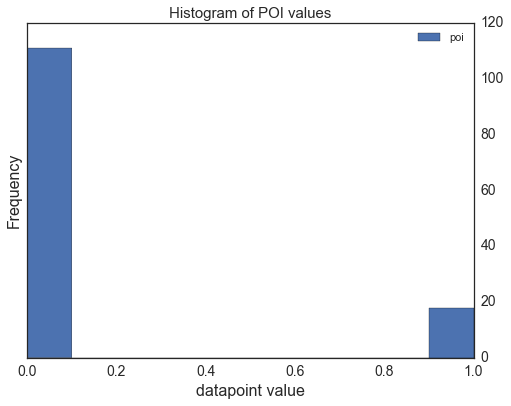
\includegraphics[width=1\textwidth]{figures/poi}
    \label{poi}}
    
    \caption{\textbf{Person of Interest plot. }\textit{The histogram shows an unbalanced target dataset with approximately 128 values of \{0: NOT POI\} and 18 values of \{1: POI\}.}}
\end{figure}


For this reason, using ``Accuracy'' as a performance metric leads to misleading information. A more apt measure of the performance of a learner should take into account the results of a confusion matrix and  calculate ``precision,'' ``recall,'' and ``$F_1$'' scores. 

For the task of identifying persons who may be involved with fraud at Enron, we will be using the $F_1$ score, i.e., the weighted average of precision and recall as our metric of choice.


%----------------------------------------------------------------------------------------
%  CHAPTER 
%----------------------------------------------------------------------------------------

\chapter*{Identify Fraud From Enron Data: Analysis}

\section*{Data Exploration}

The Enron dataset used in the project was created by the Udacity team. It was done by combining the Enron email and financial data. The data is stored in a python dictionary where each key-value pair in the dictionary corresponds to one person. For example the dictionary belows shows the corresponding key-value data point of Enron executive Pai Lou, the only executive to reap and keep substantial wealth from Enron. 

\begin{verbatim}
data_dict['PAI LOU L']
{'bonus': 1000000,
 'deferral_payments': 'NaN',
 'deferred_income': 'NaN',
 'director_fees': 'NaN',
 'email_address': 'lou.pai@Enron.com',
 'exercised_stock_options': 15364167,
 'expenses': 32047,
 'from_messages': 'NaN',
 'from_poi_to_this_person': 'NaN',
 'from_this_person_to_poi': 'NaN',
 'loan_advances': 'NaN',
 'long_term_incentive': 'NaN',
 'other': 1829457,
 'poi': False,
 'restricted_stock': 8453763,
 'restricted_stock_deferred': 'NaN',
 'salary': 261879,
 'shared_receipt_with_poi': 'NaN',
 'to_messages': 'NaN',
 'total_payments': 3123383,
 'total_stock_value': 23817930}
\end{verbatim}


\begin{itemize}%
\item financial features:\\ \texttt{salary, deferral\_payments, total\_payments, loan\_advances, bonus, restricted\_stock\_deferred, deferred\_income, total\_stock\_value, expenses, exercised\_stock\_options, other, long\_term\_incentive, restricted\_stock, director\_fees}

\item email features:\\ \texttt{to\_messages, email\_address, from\_poi\_to\_this\_person, from\_messages, from\_this\_person\_to\_poi, shared\_receipt\_with\_poi}

\item POI label:\\ \texttt{poi}

\end{itemize}

\begin{table}[!htbp]
  \begin{center}
  \caption{Persons of interest in the dataset.}
    \begin{tabular}{ l } 
    PERSONS OF INTEREST                \\ 

    \hline
    BELDEN TIMOTHY N    \\ 
    BOWEN JR RAYMOND M  \\ 
    CALGER CHRISTOPHER F\\ 
    CAUSEY RICHARD A    \\ 
    COLWELL WESLEY      \\ 
    DELAINEY DAVID W    \\ 
    FASTOW ANDREW S     \\ 
    GLISAN JR BEN F     \\ 
    HANNON KEVIN P      \\ 
    HIRKO JOSEPH        \\ 
    KOENIG MARK E       \\ 
    KOPPER MICHAEL J    \\ 
    LAY KENNETH L       \\ 
    RICE KENNETH D      \\ 
    RIEKER PAULA H      \\ 
    SHELBY REX          \\ 
    SKILLING JEFFREY K  \\ 
    YEAGER F SCOTT      \\ 
    \end{tabular}
    \label{tablePoi}
  \end{center}
\end{table}

Table \ref{tablePoi} shows a list of persons of interest that were generated by the Udacity team. This particular instance of the Enron dataset has the following characteristics:
\begin{itemize}
    \item Total number of data-points: 146
    \item Total number of POI: 18
    \item Total number of Non POI: 128
    \item Number of features used: 20
\end{itemize} 
For this dataset all features except the \texttt{`poi'} had several \textit{missing} values. From table \ref{tableFeatureMissing}, we can see that several features have more than 40+\% of their data-point values missing. In order to deal with this issue, we decided to set all missing values to `0'. 


\begin{table}[!htbp]
  \begin{center}
  \caption{A list of features with percentage missing values.}
    \begin{tabular}{ |p{5cm}|p{3cm}| } 
    \hline
    Feature Name &  \% of \textbf{Missing} Values\\[1ex]

    \hline
    poi                            & 0.0000\% \\
    bonus                          & 0.4384\% \\
    deferral\_payments              & 0.7329\% \\
    deferred\_income                & 0.6644\% \\
    director\_fees                  & 0.8836\% \\
    exercised\_stock\_options        & 0.3014\% \\
    expenses                       & 0.3493\% \\
    from\_messages                  & 0.4110\% \\
    from\_poi\_to\_this\_person        & 0.4110\% \\
    from\_this\_person\_to\_poi        & 0.4110\% \\
    loan\_advances                  & 0.9726\% \\
    long\_term\_incentive            & 0.5479\% \\
    other                          & 0.3630\% \\
    restricted\_stock               & 0.2466\% \\
    restricted\_stock\_deferred      & 0.8767\% \\
    salary                         & 0.3493\% \\
    shared\_receipt\_with\_poi        & 0.4110\% \\
    to\_messages                    & 0.4110\% \\
    total\_payments                 & 0.1438\% \\
    total\_stock\_value              & 0.1370\% \\
    \hline
    \end{tabular}
    \label{tableFeatureMissing}
  \end{center}
\end{table}

\begin{figure}[!hbtp]
\centering
    \subfloat[]{%
    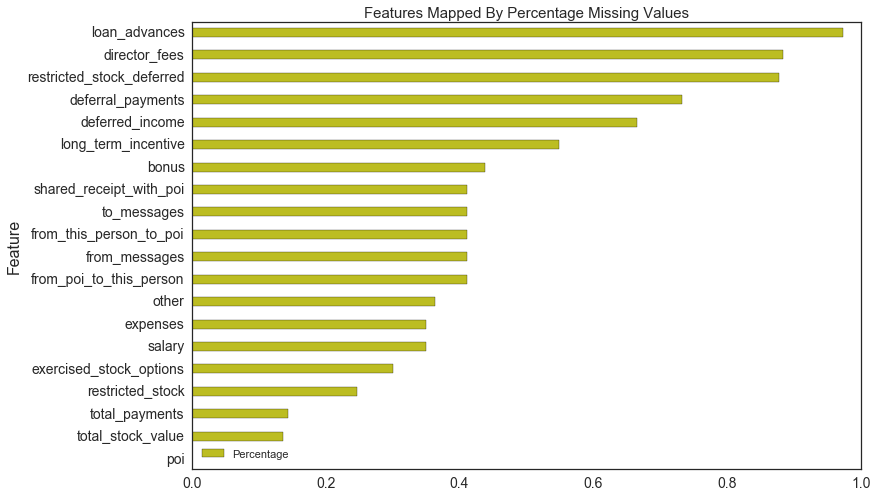
\includegraphics[width=1\textwidth]{figures/featuresByPercentageMissingValues}
    \label{featuresByPercentageMissingValues}}
    
    \caption{\textbf{Features Mapped By Percentage Missing Values. }\textit{The image shows several features with more than 40+\% of their data-point values missing.}}
\end{figure}



\clearpage

\section*{Outlier detection}
 As part of the data exploration process, we were careful to analyze the data for potential outliers. One of the first task we did was visualize the salary of Enron executives \ref{salary}. From that visualization, it was clear that there was an outlier in the dataset. We found a data-point that was completely outside of a reasonable range as can be seen from figures \ref{salary} and \ref{SalaryBonus}. 

\begin{figure}[!hbtp]
\centering
    \subfloat[]{%
    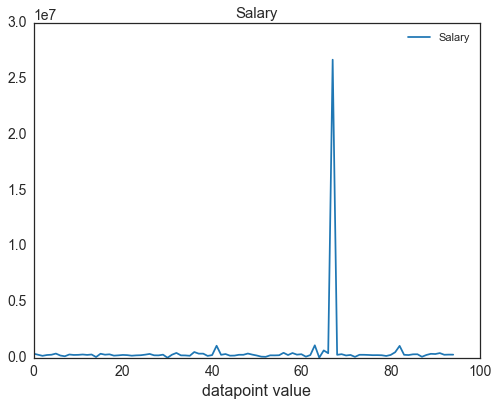
\includegraphics[width=0.6\textwidth]{figures/salary}
    \label{salary}}
    
    \caption{\textbf{Plot of Enron employee salaries.}\textit{ From this visualization, we can see there is a huge spike to the right of data-point 100, this spike corresponds with an outlier of value \$26,704,229.00.}}
\end{figure}

\begin{figure}[!hbtp]
\centering
    \subfloat[]{%
    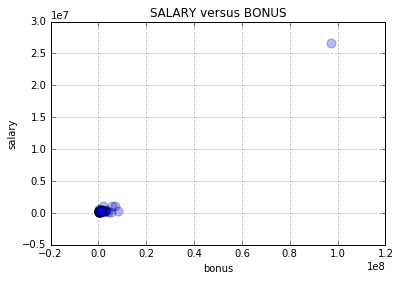
\includegraphics[width=0.6\textwidth]{figures/salary_v_bonus}
    \label{SalaryBonus}}
    \subfloat[]{%
    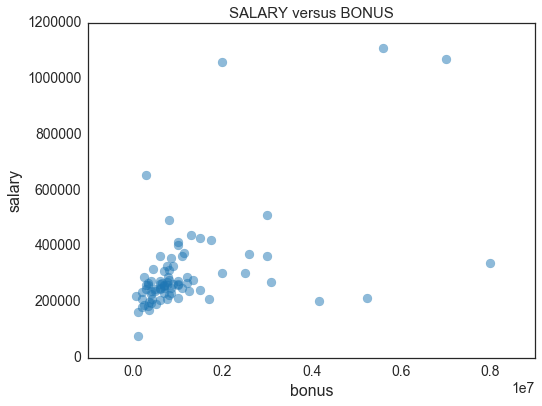
\includegraphics[width=0.6\textwidth]{figures/salary_v_bonus2}
    \label{SalaryBonus2}}
    
    \caption{\textbf{TOTAL insertion.} \textit{Figure (a) Bonus versus salary with outlier present. Figure (b) Same dataset but without the outlier. By visualizing these two features in a scatter plot we were able to clearly detect the existence of an outlier. In addition, once the data had been cleansed of outliers, we can see that majority of data-points cluster in a close range, with a few data-points spread outside bonus range of \$2 million. From descriptive statistics, we learned that the 75-percentile of bonus amount was \$1 million. }}
\end{figure}


 A closer look revealed that the data-point was an input error which included the TOTAL of all salaries as its own row. The data-point was removed leaving the dataset in a more realistic state as can be seen from figure \ref{SalaryBonus2}.




\section*{Exploratory Visualization}

One of the areas we concentrated on was that of compensation. We were very interested in the compensation packages as represented in the financial data of the executives. We moved ahead with a working hypothesis, that if fraud was indeed occurring at Enron, then more than likely, the money was probably going to be funneled out through paid bonuses and stocks. A more rigorous hypothesis would then correlate stock options granted and exercised by the Enron executives with the sales of the shares on the open market. However, such an investigation, is outside the scope of this project. 

\begin{table}[!htbp]
  \begin{center}
  \caption{Financial data on some of Enron's top paid employees.}
    \begin{tabular}{ |l|l|l| } 
    \hline
    NAME                &  SALARY        &  BONUS       \\ 

    \hline
    ALLEN PHILLIP K     &  \$201,955.00    &     4,175,000\\ 
    BELDEN TIMOTHY N    &  \$213,999.00    &     5,249,999\\ 
    SKILLING JEFFREY K  &  \$1,111,258.00  &     5,600,000\\ 
    LAY KENNETH L       &  \$1,072,321.00  &     7,000,000\\ 
    \hilight{LAVORATO JOHN J}     &  \$339,288.00    &     8,000,000\\ 
    \hline
    \multicolumn{3}{|c|}{}\\
    \hline
    NAME                &  SALARY        &  EXERCISED STOCK OPTIONS \\

    \hline
    FREVERT MARK A      &  \$1,060,932.00  &    10,433,518\\ 
    \hilight{PAI LOU L}           &  \$261,879.00    &    15,364,167\\ 
    SKILLING JEFFREY K  &  \$1,111,258.00  &    19,250,000\\ 
    RICE KENNETH D      &  \$420,636.00    &    19,794,175\\ 
    LAY KENNETH L       &  \$1,072,321.00  &    34,348,384\\ 
    \hline
    \multicolumn{3}{|c|}{}\\
    \hline
    NAME                &  SALARY        &  RESTRICTED STOCK\\ 

    \hline
    YEAGER F SCOTT      &  \$158,403.00    &     3,576,206\\ 
    IZZO LAWRENCE L     &  \$85,274.00     &     3,654,808\\ 
    BAXTER JOHN C       &  \$267,102.00    &     3,942,714\\ 
    KEAN STEVEN J       &  \$404,338.00    &     4,131,594\\ 
    FREVERT MARK A      &  \$1,060,932.00  &     4,188,667\\ 
    SKILLING JEFFREY K  &  \$1,111,258.00  &     6,843,672\\ 
    \hilight{PAI LOU L}          &  \$261,879.00    &     8,453,763\\ 
    WHITE JR THOMAS E   &  \$317,543.00    &    13,847,074\\ 
    LAY KENNETH L       &  \$1,072,321.00  &    14,761,694\\ 
    \hline
    \end{tabular}
    \label{tableSubsetEmployeeData}
  \end{center}
\end{table}

To zoom in on the compensation, we focused on three features `bonus,', `exercised\_stock\_options' and `restricted\_stock'. Table \ref{tableSubsetEmployeeData} shows some financial data for some of the highest compensated employees. It comes as no surprise that we see that the sitting CEO at the time of the collapse, Ken Lay, had the second highest bonus paid, that wasn't surprising. What was surprising was the name ``John Lavorato.'' He was the employee that got the highest bonus. So who was John Lavorato? He was the former head of Enron's trading operations. 

Another interesting character that showed up in the financial data was ``Pai Lou.'' From table \ref{tableSubsetEmployeeData}, one can see that he had some of the largest exercised stock options. Apart from the past CEOs and chairmen, he was \emph{the} employee that sold the most Enron stock. He also got some of the largest shares of restricted stock. Its interesting that these men aren't on the POI list in table \ref{tablePoi}. I firmly believe they are probably on the co-conspirators unindicted list.

To gain insights into the relationship between salary and exercised stock options, we took that subset of data and ran a KMeans clustering algorithm on it to see how the data clustered; we focused on three clustered as can be seen from figure \ref{salaryExercisedStock}. The clusters generated matched our intuition about the executives, mostly all the five executives with the highest exercised stock options were clustered as one, as can be seen in the visualization in figure \ref{salaryExercisedStock} by the markers colored blue. It is important to note we were not able to infer a relationship between salary and exercised stock options as we had thought. 

We proceeded on, with a hypothesis that more than likely, the executives with the highest salaries, probably also had the highest restricted stock. Just as with exercised stock options, it wasn't the case. From figure \ref{salaryRestrictedStock} one can see that there is a data-point with a salary close to \$200,000, but with over 8 million shares, when most of the other folks around that salary bracket had less than a million shares. Its important to note that for both our visualizations, the KMeans clustering algorithm, clustered the data-points along both the exercised stock options and restricted stocks. 
\begin{figure}[!hbtp]
\centering
    \subfloat[]{%
    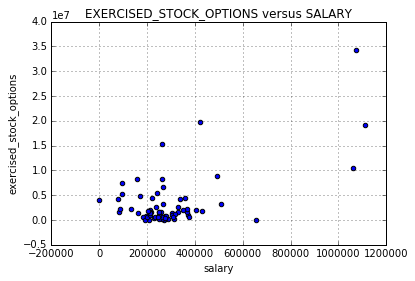
\includegraphics[width=0.6\textwidth]{figures/salary_v_exercised_stock_options}
    \label{salaryExercisedStock}}
    \subfloat[]{%
    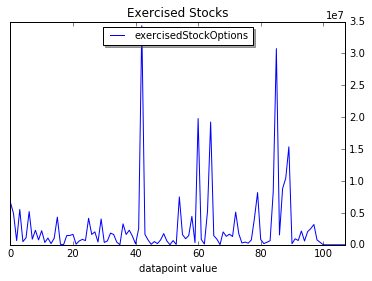
\includegraphics[width=0.6\textwidth]{figures/exercised_stock_options}
    \label{salaryExercisedStock2}}
    
    \caption{\textbf{A closer look at salary and exercised stock options.} \textit{Figure (a) A scatter plot of salary versus exercised stock options. Figure (b) A plot of exercised stock options. From these two plots one can see that there is a small subset of senior executives who exercised a significant amount of Enron shares. }}
\end{figure}

\begin{figure}[!hbtp]
\centering
    \subfloat[]{%
    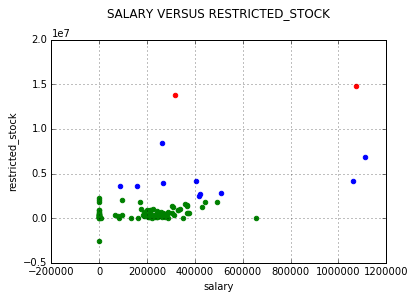
\includegraphics[width=0.6\textwidth]{figures/salary_v_restricted_stock}
    \label{salaryRestrictedStock}}
    \subfloat[]{%
    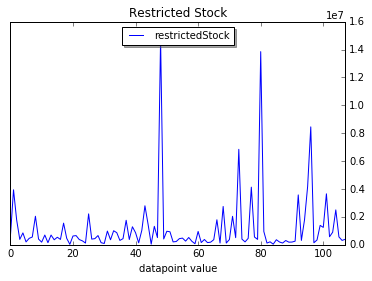
\includegraphics[width=0.6\textwidth]{figures/restricted_stock}
    \label{salaryRestrictedStock2}}
    
    \caption{\textbf{A closer look at salary and restricted stock.} \textit{A scatter plot of salary versus restricted stock. Figure (b) A plot of restricted stock.}}
\end{figure}

\clearpage
\section*{Algorithms and Techniques}

For the problem of identifying fraud from the Enron financial and email data, we experimented with four different classifiers, three ensemble methods and a regression:
\begin{enumerate}% 
\item A RandomForestClassifier\\
We selected this learner because it is considered one of the best off-the-shelf learning algorithm, and requires almost no tuning. 
\item An ExtraTreesClassifier\\
 Its another ensemble learner like Random Forest, with one caveat. When creating a branch in a tree, Random Forest chooses the most discriminant value, whereas ExtraTrees split point is arbitrarily. This helps to increase the bias slightly and lower the variance even more.
\item An eXtreme Gradient Boosted (XGBoost) Trees Classifier\\
XGBoost is an advanced implementation of gradient boosting algorithm. From reading literature on machine learning in practice, the XGBoost classifier has differentiated itself as a classifier that is amenable to wide range of problems from particle physics, to ad click through rate prediction and so on. For example, ``among the 29 challenge winning solutions published at Kaggle's
blog during 2015, 17 solutions used XGBoost'' \cite{ChenG16}. As a result, we also wanted to see if using this classifier could give us good results with our dataset.

\item A LogisticRegression (Robust, with $Lp$ = $L1$) Classifier\\
Its computational simpler than the ensemble methods. Furthermore, it has been used in real life to predict adverse risk events that have relatively small chances of occurring like credit card fraud and so on. The dataset composition of those events are similar to the Enron dataset, where the labels are heavily skewed towards one class. Another reason we selected the robust LogisticRegression based on the fact that it handles outliers better. While the data has been cleansed of ``outliers,'' there are a few executives whose data-points fall outside of the mean by several standard deviations.

\end{enumerate}



\section*{Benchmark}

For this specific problem, we were unable to acquire benchmarks that we could test the performance of our learners against. However in the notes accompanying the project description, we were tasked to shoot for a precision score of over 0.3. From our four learners, and the initial trials, we have already superseded this number, as can be seen from table \ref{tableBenchMarkScores}.


%----------------------------------------------------------------------------------------
%  CHAPTER 
%----------------------------------------------------------------------------------------
\chapter*{Identify Fraud From Enron Data: Methodology}

\section*{Data Preprocessing}
Significant data preprocessing wasn't necessary for this problem. Once we cleared our dataset of outliers, we decided to play with a few features to get a feel of how they would behave with the algorithms. 

We tested out our four learners with \texttt{salary} and \texttt{bonus} features before we scaled them with a minimax-scaler afterwards. We found no difference, so we decided to forgo scaling.

We dropped the feature named \texttt{email\_address} from our dataset because it contained a string, while other features where numeric. Furthermore, we felt that this feature was superfluous with respect to the task. 

\section*{Feature Engineering}
We suspected that there was interdependence of features so we engineered a feature, the ``fraction of emails to and from poi.'' We figured this metric could give us another window into discriminating the data. 

\section*{Feature Selection}
Our approach to feature selection was based on intuition as well as running the features through feature selection algorithms to guide us in our decision of features to use. In the case of the latter we selected a RandomForest classifier as well as a Gradient Boosted Trees---XGBoost---classifier to implement feature selection.

For the RandomForest algorithm, we used a baseline classifier, we fitted it to our data and used its ``\texttt{feature\_importances\_}'' function to obtain a score on the strength of that feature. To obtain reliable scores, we ran the algorithm a 1000x and averaged the scores of the features to obtain the top $n$ features as visualized in figure \ref{randomForestFeatureImportance}.

\begin{figure}[!hbtp]
\centering
    \subfloat[]{%
    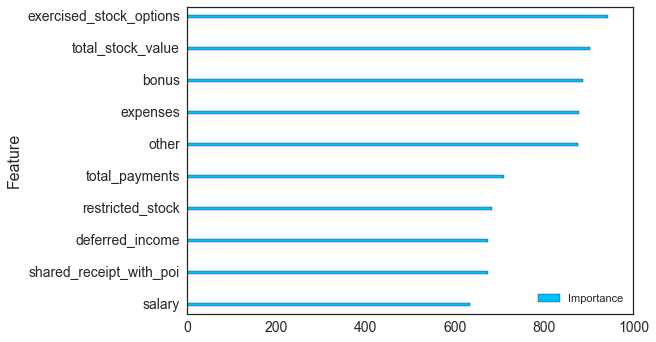
\includegraphics[width=1\textwidth]{figures/randomForestFeatureImportance}
    \label{randomForestFeatureImportance}}
    
    \caption{\textbf{Feature importance as discovered by RandomForest.} \textit{}}
\end{figure}

For the XGBoost classifier, we took a different approach to obtaining reliable data. We re-sampled the dataset and grew it a 1000x using sklearn's \texttt{StratifiedShuffleSplit} function with a thousand folds. We then fed this more expansive dataset to an \texttt{XGBoost} classifier and applied its \texttt{plot\_importance} function to discover the important features as can be seen from figure \ref{xgboostFeatureImportance}.

\begin{figure}[!hbtp]
\centering
    \subfloat[]{%
    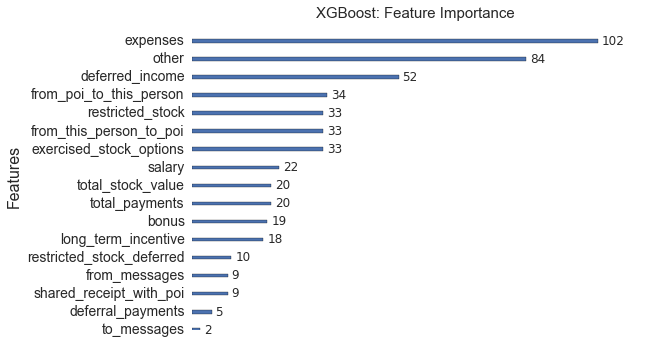
\includegraphics[width=1\textwidth]{figures/xgboostFeatureImportance}
    \label{xgboostFeatureImportance}}
    
    \caption{\textbf{Feature importance as discovered by XGboost.} \textit{}}
\end{figure}


\setlength{\extrarowheight}{1.5pt}
\begin{table}[!htbp]
\caption{Scores} %title of the table
\centering % centering table
\begin{tabular}{|p{6cm}|p{1.5cm}|p{1.5cm}|p{1.5cm}|} % creating four columns
\hline % inserts single-line
\multicolumn{4}{|c|}{}\\
\multicolumn{4}{|c|}{Result of Training with \textbf{RandomForest} generated features}\\[5pt]
\hline 
& \multicolumn{3}{c|}{Metrics}\\[5pt]
\cline{2-4} 
& Precision & Recall & F1\\[0.5ex]
\hline % inserts single-line

ExtraTreesClassifier     &  0.387       &  0.144     &  0.210     \\ 
LogisticRegression       &  0.416       &  0.170     &  0.241     \\ 
RandomForestClassifier   &  0.370       &  0.140     &  0.203     \\ 
XGBClassifier            &  0.441       &  0.200     &  0.275     \\ 


\hline% inserts single-line

\multicolumn{4}{|c|}{}\\
\multicolumn{4}{|c|}{Result of training with \textbf{XGBoost} generated features}\\[5pt]
\hline 
& \multicolumn{3}{c|}{Metrics}\\[5pt]
\cline{2-4} 
& Precision & Recall & F1\\[0.5ex]
\hline % inserts single-line

ExtraTreesClassifier     & 0.454       & 0.174     & 0.252\\     
LogisticRegression       & 0.293       & 0.200     & 0.237\\     
RandomForestClassifier   & 0.379       & 0.131     & 0.194\\     
XGBClassifier            & 0.416       & 0.196     & 0.266\\

\hline% inserts single-line

\multicolumn{4}{|c|}{}\\
\multicolumn{4}{|c|}{Result of training with \textbf{Ad-hoc} features}\\[5pt]
\hline 
& \multicolumn{3}{c|}{Metrics}\\[5pt]
\cline{2-4} 
& Precision & Recall & F1\\[0.5ex]
\hline % inserts single-line

ExtraTreesClassifier     &  0.449       &  0.140     &  0.213     \\ 
LogisticRegression       &  0.499       &  0.169     &  0.252     \\ 
RandomForestClassifier   &  0.404       &  0.146     &  0.215     \\ 
\hilight{XGBClassifier}  &  \hilight{0.422} &  \hilight{0.299} &  \hilight{0.350}     \\ 

\hline % inserts single-line

\end{tabular}
\label{tableBenchMarkScores}
\end{table}

We used these features selected by the algorithms along side our domain guided features on our four baseline learners, the results can be see in table \ref{tableBenchMarkScores}. From this experiment, we decided to go with our ad-hoc generated features because the performance was superior when we considered the $F_1$ score of all four learners. It is important to note that the other features were not woeful in their performance, and overall, these features with baseline classifiers had already put us over the threshold of the benchmark precision score---0.3---we were to surpass.

For the final algorithm, we ended up going with our intuition and selecting features that we had explored in the data analysis. These features are as follows: 
\begin{verbatim}
poi
bonus
exercised_stock_options
restricted_stock
fraction_from_poi
fraction_to_poi
from_poi_to_this_person
from_this_person_to_poi
salary
\end{verbatim}


\section*{Implementation}

We implemented the four learning algorithms. For each of the learners we implemented the baseline algorithm using a stratified shuffle split cross validation with a thousand folds and calculated the precision, recall and $F_1$ scores respectively.


\section*{Refinement}
To improve on the performance of the algorithm, we decided to reduce the number of features that were used for training. Through some trial and error, we realized if we held the feature list to the first three features:
\begin{verbatim}
bonus
exercised_stock_options
restricted_stock 
\end{verbatim}
Our performance improved dramatically as can be seen in table \ref{tableReducedFeatures}.

\section*{Parameter Tuning}

\textbf{Question} Discuss parameter tuning and its importance.

Parameter tuning is the process of discovering \emph{optimal} choices for the hyper-parameters that support a model. These hyper-parameters are parameters that are not part of the \emph{core} specifications for describing a model as a mathematical function, i.e., they are not \emph{learned} during the training phase.

These \emph{hyper}-parameters are the keys we turn that allow us to control for over-fitting. They are the tools we use to restrict the capacity of our models, i.e., how flexible the model can be. These parameters influence to a large extent either the accuracy and or speed of a model. 

There are several approaches to \emph{tuning} these parameters, most of them can be considered as a search through some hyper-parameter space. Finding these parameters then becomes finding the right combinations that optimize the performance metric we are interested in optimizing for. The usual way to do that is through a grid search, a randomized grid search or smart tuning. 



Once we settled on the features we would be using for our classification task, we tuned our model using sklearn's \texttt{GridSearch} in conjunction with a \{k=1000 fold\} \texttt{StratifiedShuffleSplit} function, we tuned both the tree parameters as well as the task parameters of our XGBoost classifier to control for over-fitting and improve over all performance. The parameters we tuned are as follows:

\begin{itemize}
\item Parameters for Tree Booster
    \begin{itemize}
        \item \texttt{max\_depth}
        \begin{itemize}
            \item Maximum depth of tree
            \item Range [1, $\infty$], default 6, tuned on $[3,5,7]$
        \end{itemize}
        \item \texttt{minimum\_child\_weight}
        \begin{itemize}
            \item Minimum sum of instance weight needed in children
            \item Range $[0,\infty]$ default 0, tuned on $[1,3,5]$
        \end{itemize}
        \item \texttt{max\_delta\_step}
        \begin{itemize}
            \item Maximum delta step that each trees weight is allowed to be
            \item Range $[0, \infty]$ default 0, tuned on $[0, 1, 2]$
        \end{itemize}
    \end{itemize}

\item Task Parameter
    \begin{itemize}
        \item \texttt{learning\_rate}
        \begin{itemize}
            \item Scale the contribution of each tree by learning rate
            \item Range $[0, 1]$, tuned on $[0.01, 0.1, 0.02, 0.2, 0.25, 0.3]$
        \end{itemize}
    \end{itemize} 
\end{itemize}

Once we performed our search through the hyper-parameter space to find the combination of hyper-parameters that maximized the performance of our classifier, we were able to improve the previous $F_1$ score by 7.2\%. Here is the final model for classifying persons of interest in the Enron fraud case.
\begin{verbatim}
XGBClassifier(base_score=0.5, colsample_bylevel=1, colsample_bytree=1,
       gamma=0, learning_rate=0.02, max_delta_step=1, max_depth=3,
       min_child_weight=1, missing=None, n_estimators=100, nthread=-1,
       objective='binary:logistic', reg_alpha=0, reg_lambda=1,
       scale_pos_weight=1, seed=0, silent=True, subsample=1)
\end{verbatim}



\section*{Validation}

\textbf{Question} Discuss validation and its importance.

\textbf{Answer} When the learning algorithm is in the process of discovering the ideal function which describes the data, in order to prevent over-fitting, we hold out a piece of the data and use it as a \textbf{test} set. This is what is meant by validation. 

If \texttt{GridSearchCV} is used to optimize hyper-parameters in our model, and we test those hyper-parameters out on the \textbf{test} set, information from that sample can eventually leak into our model, which reduces its ability to generalize. As a means of preventing this, a sample of the data is held out in an \textbf{evaluation} set which the algorithm tests on. 

Each combination of parameters is evaluated against this evaluation set. A method of doing this is called \textbf{cross validation}, i.e., a process of testing out hyper-parameter optimization on a data sample that is independent of both the testing and training data.

In the case of \textbf{K-fold CV} the data set is divided into $k$ subsets, and the holdout method is repeated $k$ times. Each time, one of the $k$ subsets is used as the test set and the other $k-1$ subsets are put together to form a training set. Then the average error across all $k$ trials is computed. The advantage of this method is that it matters less how the data gets divided. Every data point gets to be in a test set exactly once, and gets to be in a training set $k-1$ times. Once the hyper-parameters are optimally tuned, one can test the efficacy of the final model on the test set. 

In our case with a small-\emph{highly}-skewed dataset, K-fold cross validation is especially useful when used in conjunction with \texttt{GridSearchCV}. We know that the final parameters that result from the process are those that accurately optimize the performance metric. 

To validate our model, we used sklearn's \texttt{StratifiedShuffleSplit} using \{k=1000\}. We trained our four models on the reduced features we found through trial and error and recorded their performance. 


\section*{Model Evaluation}

To evaluate the performance of our algorithms, we used the following metrics:
\begin{enumerate}
\item Precision 
\item Recall 
\item $F_1$ score
\end{enumerate}

From our trials we recorded the scores for each of our metrics as can be seen in table \ref{tableReducedFeatures}. 

The LogisticRegression had the highest precision score. With regards to this dataset, it means that whenever a POI gets flagged in the test set, we know with a lot of confidence that it's very likely to be a real POI and not a false alarm. On the other hand, it had a low recall score, which means that sometimes it misses real POIs.  

While the XGBClassifier did not have the highest precision score, it had the highest recall score. This means that nearly every time a POI is in the test set, we are able to classify them. 

Furthermore, the XGBClassifier had the best $F_1$ score. For this problem, this is the best we can do. Both the false positive and false negative rates are relatively low, which means that the model can identify POI's reliably and accurately. As a result the \textbf{XGBClassifier} was the most apt model for this problem.



\setlength{\extrarowheight}{1.5pt}
\begin{table}[!htbp]
\caption{Result of training with reduced features} %title of the table
\centering % centering table
\begin{tabular}{|p{6cm}|p{1.5cm}|p{1.5cm}|p{1.5cm}|} % creating four columns
\hline % inserts single-line
& \multicolumn{3}{c|}{Metrics}\\[5pt]
\cline{2-4} 
& Precision & Recall & F1\\[0.5ex]
\hline % inserts single-line

ExtraTreesClassifier     &  0.490       &  0.181     &  0.264     \\ 
LogisticRegression       &  0.630       &  0.202     &  0.306     \\ 
RandomForestClassifier   &  0.483       &  0.190     &  0.272     \\ 
XGBClassifier            &  0.505       &  0.332     &  0.400     \\ 
\hline% inserts single-line

\multicolumn{4}{|c|}{}\\
\multicolumn{4}{|c|}{Result of tuning the \textbf{XGBoost} classifier}\\[5pt]
\hline
& \multicolumn{3}{c|}{Metrics}\\[5pt]
\cline{2-4} 
& Precision & Recall & F1\\[0.5ex]
\hline % inserts single-line

XGBClassifier           &  0.617  & 0.331  & 0.431\\ 
\hline
\end{tabular}
\label{tableReducedFeatures}
\end{table} 

%----------------------------------------------------------------------------------------
%  CHAPTER 
%----------------------------------------------------------------------------------------

\chapter*{Identify Fraud From Enron Data: Conclusion}


\section*{Reflection}

We have presented a solution to identifying ``persons of interest'' who \textit{might} have played a significant role in perpetuating fraud at Enron from their finance and email data. 

We begun our solution by reading about the fraud and watching a couple of documentaries around it to understand the context in which the problem occurred. We then proceeded by doing a rigorous analysis on the dataset. 

The first thing we noticed was the skew of the dataset towards negative examples of persons of interest. From this discovery we realized we would need to pay careful attention to the metrics of performance we used for choosing the appropriate algorithm. In most cases, ``Accuracy'' of the classifier would be considered a \textit{good} metric to use, but because of the imbalance in the data, a combination of both the ``precision'' and ``recall'' as realized in the ``$F_1$'' score was the more apt choice.

From our analysis we discovered some outliers and removed them from the dataset. We took a close look at ``exercised stock options'' and ``restricted stocks'' to see how the senior executives were compensated. Based on our working hypothesis that if fraud was indeed been fomented at Enron, then more than likely the vehicle that the senior officers would take to get the money out would be through an inflated allocation of shares. 

We selected three ensemble learners (Random Forest, Extra Trees, eXtreme Gradient Boosted Trees) and one regression (Robust) as algorithms to explore in discriminating this dataset. We selected these algorithms for their ease of interpret-ability with respect to understanding which features played the most important role is classifying the data. Since we didn't have existing benchmarks we could use to reason about the effectiveness of our approach, we resorted to using the precision benchmark of a score over 0.3 as the goal to surpass.

We experimented with feature selection algorithms, but eventually went with ad-hoc features that we selected based on intuition on domain knowledge. From our learning experiments we selected the eXtreme Boosted Trees classifier as the learner to use. We reduced our feature space and tuned our classifier to achieve this final score, \{$F_1$: 0.431, precision: 0.617, recall: 0.331\}.

\section*{Improvement}
One of the more interesting aspect of this project was the selected features that were used for the final classifier; all those features came from the financial data. When we took away the feature that we engineered from the email data as well as other features from the email data, we got an increase in performance. 

We believe we could get more additive data from the Enron emails by performing some natural language understanding techniques and then adding those features to the dataset.

With respect to the algorithms used, there a definite ways these algorithms could be improved upon. We only optimized for four hyper-parameters for our eXtreme Gradient Boosted trees. That algorithm has many more hyper-parameters that could yield a stronger model.

If time was not a factor, we could create a pipeline that used Grid Search to go through a combination of features while optimizing the XGBoost algorithm for its own hyper-parameters. We could do an exhaustive search of this feature + hyper-parameters space to obtain a model that would be most optimal for describing this data.



%--------------------------------------------------------------------------------
%  REFERENCE LIST
%--------------------------------------------------------------------------------
\vspace{4\baselineskip}\vspace{-\parskip} % Creaters proper 4 blank line spacing.
\footnotesize % Makes bibliography 10 pt font.
\bibliographystyle{unsrtnat} %Can use a different style as long as it is one which uses numbered references in the text.
\bibliography{ml}





\end{document}




